\chapter{前言}
\section{应用背景:协同编辑应用}
	\par 协同编辑系统,可以允许不同地点的用户同时编辑同一份文档。为了获得较快的响应和较高的实用性,系统会在不同的地点或设备进行文档的复制。一个用户可以在某个副本上进行文档的编辑,并将做出的修改异步地传递给其他副本。不必要等待服务器处理完再响应用户操作,本地操作可以立即执行。同时系统必须保证编辑的一致性,即在所有用户完成文档的编辑后,所有的副本内容一致。
\begin{figure}
\centering
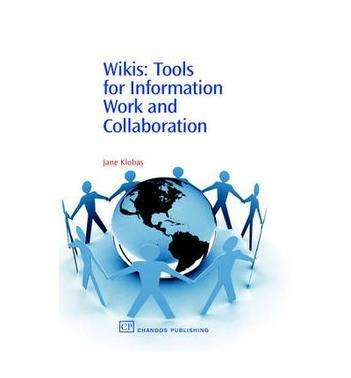
\includegraphics{figures/timg.jpg}
\caption{系统编辑实例}
\label{fig:graph}
\end{figure}
\section{技术背景:Replicated List 规约及其基于OT的 Replicated List 算法}

\section{本文研究工作: 面向 Redis List的OT函数的设计、验证与实现}
	\par 本次毕业设计的目标是实现Redis List所支持的14种非阻塞操作的OT(Operational Transformation)函数,并且对实现函数的正确性进行验证。阿里云和RedisLab的团队目前都在对Redis List的操作进行开发,Redis List操作的OT函数实现具有应用前景和商业前途。
\section{论文组织}
	\par 本文后续内容组织如下:
	\par 第2章介绍本文的相关工作,包括系统模型和已有的相关OT函数的设计。
	\par 第3章介绍了Redis列表相关的基本命令,并对其进行了分类,然后进行了对应OT函数的设计。
	\par 第4章介绍了TLA+,并使用TLA+完成了对上述设计好的OT函数的验证。
	\par 第5章分析实验结果,并对实验结果进行分析。
	\par 第6章是本论文的结论和以后工作的相关展望。